\section{Projekt}

In dem Projekt "`Home-Bacon"' wollen wir das Thema Lokalisation mittels Bluetooth-Beacons auf Smartwatches untersuchen und als Prototyp implementieren.

\subsection{Ergebnis}
Das Ergebnis unseres Projekts sind zwei mobile Applikationen, wobei die eine für ein Android-Smartphone und die andere für eine Android-Smartwatch entwickelt wurde.

\subsection{Anwendungsfälle}
\label{sec:useCases}
Wir möchten unsere Projektidee und unsere Anforderungen in Form von User-Storys und Anwendungsfällen konkretisieren. Dazu haben wir uns den fiktiven Anwender Anton ausgedacht, der sehr vergesslich aber experimentierfreudig ist. Als technikaffiner Mensch hat Anton natürlich eine moderne Smartwatch und ein Smartphone. Aufgrund seiner Vergesslichkeit wünscht sich Anton die Möglichkeit, beim Verlassen eines Raums an bestimmte Dinge erinnert zu werden. Beispielsweise möchte er beim Verlassen des Hauses an seine Einkaufsliste erinnert werden.

Nachfolgend werden Antons Wünsche detaillierter ausgeführt.

\subsubsection{Positionierung}
Als Anwender Anton möchte ich meine eigene Position in meinem Haus bestimmen können, um zu wissen, in welchem Raum ich mich befinde. 

\begin{figure}[H]
\centering
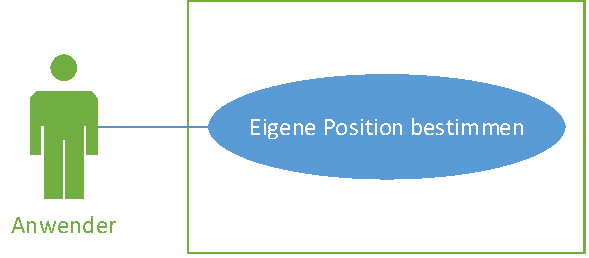
\includegraphics[width=0.54\linewidth]{Bilder/UseCase-Position}
\caption{Anwendungsfalldiagramm Positionierung}
\label{fig:UseCase-Position}
\end{figure}

\subsubsection{Notizen}
Als Anwender Anton möchte ich über mein Smartphone Notizen im aktuellen Raum anbringen können, um diese zur späteren Ansicht zu hinterlassen.

\begin{figure}[H]
\centering
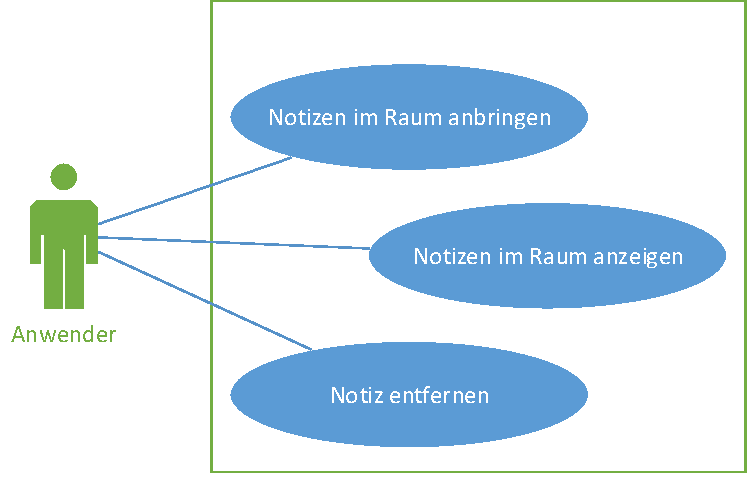
\includegraphics[width=0.7\linewidth]{Bilder/UseCase-Notizen}
\caption{Anwendungsfalldiagramm Notizen}
\label{fig:UseCase-Notizen}
\end{figure}

Darüber hinaus bekomme ich die im aktuellen Raum hinterlassenen Notizen auf meiner Smartwatch angezeigt und kann mithilfe der horizontalen Wischgeste durch diese navigieren. Außerdem möchte ich Notizen löschen können.

\subsubsection{Ereignisse}
Als Anwender Anton möchte ich Ereignisse mit Notizen verknüpfen und beim Verlassen bzw. Betreten eines Raums diese auf meiner Smartwatch sehen.

\begin{figure}[H]
\centering
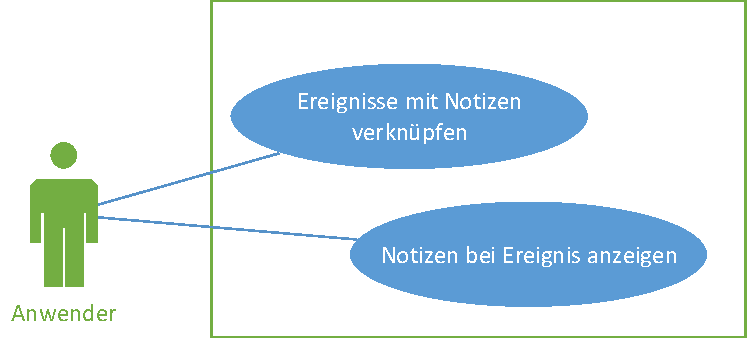
\includegraphics[width=0.7\linewidth]{Bilder/UseCase-Ereignisse}
\caption{Anwendungsfalldiagramm Ereignisse}
\label{fig:UseCase-Ereignisse}
\end{figure}

\subsection{Projektplan}
Zu Beginn unseres Projekts haben wir uns Gedanken über mögliche Projektphasen gemacht. In folgendem Diagramm haben wir unsere Zeitplanung für das Projekt aufgezeichnet.

\begin{figure}[tbh]
\centering
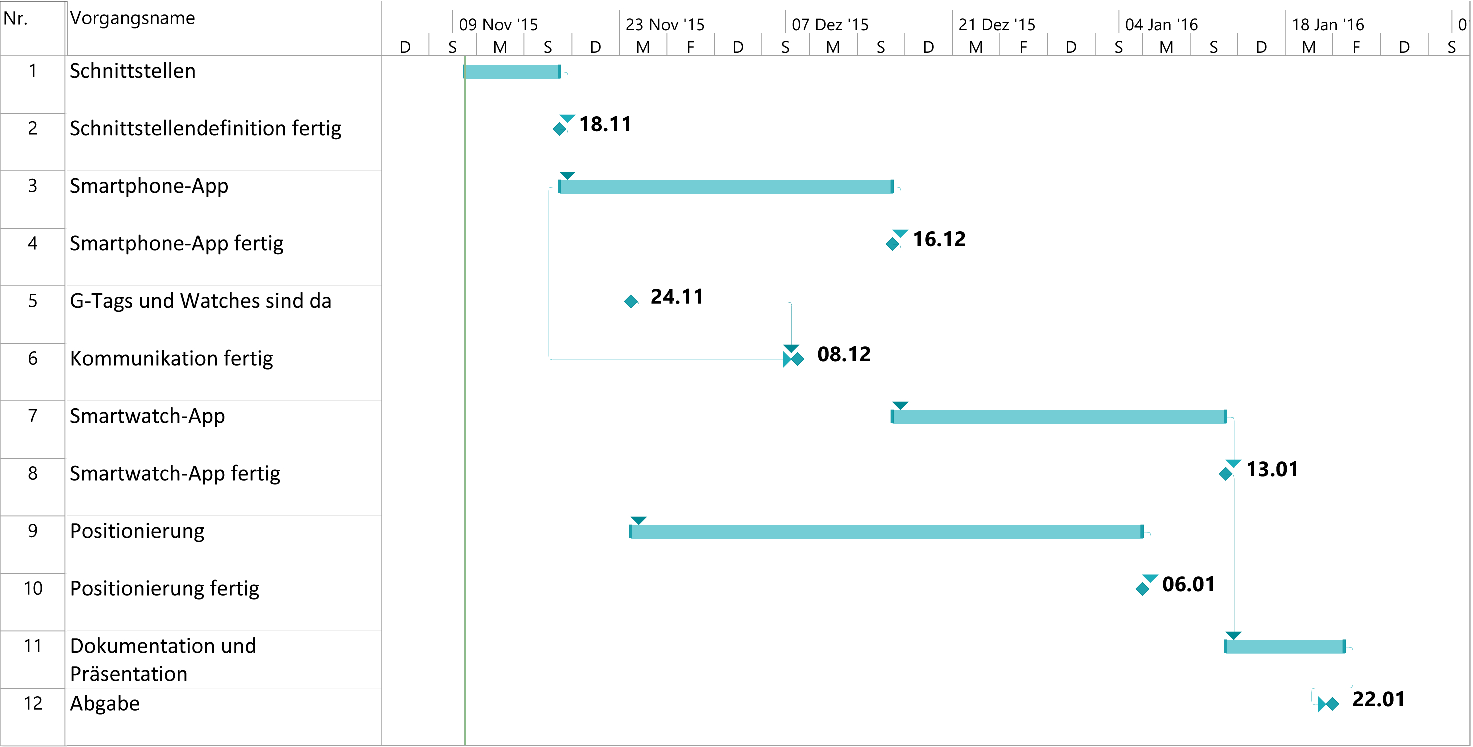
\includegraphics[width=1.0\linewidth]{Bilder/Projektplan}
\caption{Zeitplan mit Meilensteinen}
\label{fig:Zeitplan-1}
\end{figure}

\subsubsection{Projektphasen}
\begin{description}
	\item[Schnittstellen:] Definition der Schnittstellen zur Positionsbestimmung und zur Kommunikation zwischen
	Smartphone und Smartwatch. Dadurch können gewisse Teile unabhängig voneinander entwickelt werden.
	\item[Smartphone-App:] Entwicklung der Smartphone-App zur Hinterlegung von Notizen in Räumen und bei Ereignissen.
	\item[Smartwatch-App:] Entwicklung der Smartwatch-App zur Anzeige von Notizen in Räumen und bei Ereignissen.
	\item[Positionierung:] Bestimmung der Position der Smartwatch anhand der Bluetooth-Signale der stationären Bluetooth-Beacons.
	\item[Dokumentation und Präsentation:] Erstellung der Dokumentation und Vorbereitung der Präsentation.
\end{description}

\subsubsection{Meilensteine}
\begin{enumerate}
	\item Schnittstellen sind festegelegt.
	\item Geschätzter Termin für das Eintreffen der bestellten Bluetooth-Beacons und Smartwatches.
	\item Kommunikation vom Smartphone zur Smartwatch und umgekehrt ist implementiert.
	\item Die Smartphone-App ist fertig (ggf. Mock-Implementierungen für die Schnittstellen)
	\item Die Positionierung auf der Smartwatch ist fertig.
	\item Die Smartwatch-App ist fertig.
	\item Die Dokumentation wurde abgegeben.
\end{enumerate}